Chapter~\ref{ch:4_approach} has presented the final Power model that resulted from a series of experiments conducted on the model's Texter, Ruler and Aggregator components. This chapter explains and evaluates those experiments and compares the results to the final model. Section~\ref{sec:5_experiments/1_base_datasets} introduces the basic knowledge graphs and text sets that form the base for the \emph{Power datasets} presented in~\ref{sec:5_experiments/2_power_datasets}, which are then used to train and evaluate Power's Texter, Ruler and Aggregator components as shown in sections~\ref{sec:5_experiments/4_texter},~\ref{sec:5_experiments/5_ruler} and~\ref{sec:5_experiments/6_aggregator}.
In particular section~\ref{sec:5_experiments/4_texter} discusses various variations of the model that are divided into experiments with static and contextual word embeddings, the latter of which are used in the final Power model. The Texter and Ruler components are evaluated individually and, finally, as part of the Power as a whole.


\section{Base Datasets}
\label{sec:5_experiments/1_base_datasets}
Training and evaluation of a knowledge graph completion model fundamentally require a knowledge graph. In case of the Power model, there is also the need for textual entity descriptions. The graphs chosen for this work are the popular FB15K-237~\cite{Toutanova2015ObservedVL} subset of the  Freebase~\cite{Bollacker2008FreebaseAC} graph and the CoDEx~\cite{Safavi2020CoDExAC} graph, a knowledge graph constructed with the aim of providing an improved benchmark for knowledge graph completion. The texts are provided by Felix Hammann as part of his work on KGC~\cite{}, together with matching fact splits of the mentioned graphs. The following Subsections~\ref{subsec:5_experiments/1_base_datasets/1_knowledge_graphs} and~\ref{subsec:5_experiments/1_base_datasets/2_text_sets} give an impression of the size of the knowledge graphs, the shape of the fact splits and the kind of texts in the text sets.

\subsection{Knowledge Graphs}
\label{subsec:5_experiments/1_base_datasets/1_knowledge_graphs}
One of the most popular knowledge graphs is Freebase~\cite{Bollacker2008FreebaseAC}. Although it is not maintained anymore since it was integrated into Wikidata in 2015~\cite{Tanon2016FromFT}, the benchmark datasets derived from it are still widely used. One of those benchmark datasets is the \emph{FB15k} dataset introduced by Bordes et al. in 2013~\cite{Bordes2013TranslatingEF}, which covers roughly \num{15000} Freebase entities. On its basis, Toutanova and Chen introduced the FB15k-237 subset in 2015~\cite{Toutanova2015ObservedVL}, whose purpose was to create a more meaningful benchmark by eliminating trivially predictable facts. For example, if FB15k-237 covers a relation like $(x, contains, y)$, it does not include its inverse relation $(y, part~of, x)$, because good performance resulting from such trivial, mutual predictions detracts from more interesting cases. In 2020, Safavi and Koutra published another dataset called CoDEx~\cite{Safavi2020CoDExAC}, which is derived from FB15k-237 and two other datasets, covers more diverse content and in turn poses a greater challenge than FB15k and FB15k-237. From the three provided variants of the CoDEx dataset -- CoDEx-S, CoDEx-M, and CoDEx-L -- the IRT approach by Hamann, on which this work is based, focuses on the CoDEx-M dataset. \autoref{tab:5_experiments/1_data_sources/1_knowledge_graphs/benchmark_datasets} gives an overview of the scales of FB15k, FB15k-237 and CoDEx-M. CoDEx-M actually contains additional, negative facts that are excluded here as this work focuses on the common open-world scenario.

\begin{table}[h]
    \centering
    \begin{tabular}{| l | r | r | r | r | r |}
    \hline

    \multicolumn{1}{|c|}{\textbf{Dataset}} &
    \multicolumn{1}{|c|}{\textbf{#Entities}} &
    \multicolumn{1}{|c|}{\textbf{#Relations}} &
    \multicolumn{3}{|c|}{\textbf{#Facts}} \\

    \multicolumn{1}{|c|}{} &
    \multicolumn{1}{|c|}{} &
    \multicolumn{1}{|c|}{} &
    \multicolumn{1}{|c|}{\textbf{Train}} &
    \multicolumn{1}{|c|}{\textbf{Valid}} &
    \multicolumn{1}{|c|}{\textbf{Test}} \\

    \hline \hline

    FB15k     & \num{14951} & \num{1345} & \num{483142} & \num{50000} & \num{59071} \\
    FB15k-237 & \num{14541} & \num{237}  & \num{272115} & \num{17535} & \num{20466} \\
    CoDEx-M   & \num{17050} & \num{51}   & \num{185584} & \num{10310} & \num{10311} \\

    \hline
\end{tabular}

    \caption{Comparison of popular KGC benchmark datasets}
    \label{tab:5_experiments/1_data_sources/1_knowledge_graphs/benchmark_datasets}
\end{table}

As for the above KGC benchmark datasets, a graph's fact set is usually further split into training, validation, and test subsets. Thereby, the splits are created so that there are training, validation, and test facts for possibly every entity. In contrast to that common approach, in his work on zero-shot learning, Hamann creates new \emph{IRT splits} from FB15k-237 and CoDEx-M that distinguish between so-called \emph{closed-world (CW) entities}, that are seen during training, and \emph{open-world (OW) entities}, which are not seen during training, to optimize prediction for unknown entities.

\begin{figure}
    \centering
    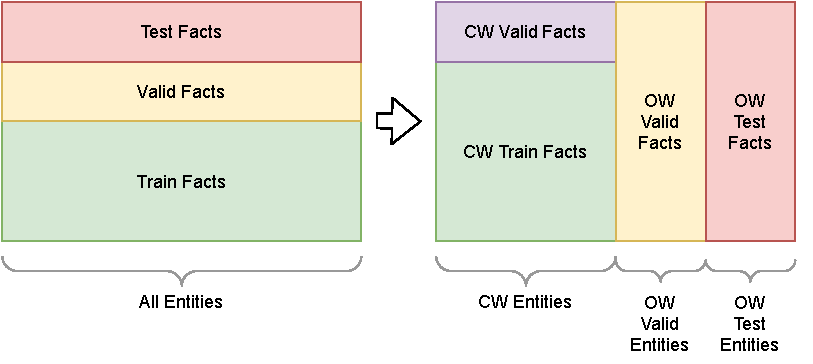
\includegraphics[width=\textwidth]{5_experiments/1_data_sources/1_knowledge_graphs/irt_split}
    \caption{Difference between a conventional and an IRT fact split. The IRT fact split focuses on open-world entities that must stay unseen during training. ``CW'' = ``closed-world'', ``OW'' = ``open-world''.}
    \label{fig:5_experiments/1_data_sources/1_knowledge_graphs/irt_split}
\end{figure}

\autoref{fig:5_experiments/1_data_sources/1_knowledge_graphs/irt_split} illustrates the different shape of an IRT fact split compared to a conventional one: The closed-world entities' facts are split into closed-world training and closed-world validation facts to enable closed-world prediction. Meanwhile, the open-world entities' facts are completely reserved for validation and training, respectively. Closed-world training and closed-world validation facts only refer to closed-world entities. On the other hand, one of an open-world validation fact's head or tail may also be a closed-world entity, and one of an open-world test fact's head or tail may be a closed-world entity or an open-world validation entity. \autoref{tab:5_experiments/1_data_sources/1_knowledge_graphs/irt_splits} gives an overview of the scales of the IRT splits' entity and fact subsets.

\begin{table}[h]
    \centering
    \begin{tabular}{ l c r r r c r r c r r }
    \toprule
    
    \multicolumn{1}{l}{\textbf{Graph}} & \phantom &
    \multicolumn{1}{c}{\textbf{\thead{CW \\ Train \\ Ents}}} &
    \multicolumn{1}{c}{\textbf{\thead{CW \\ Train \\ Facts}}} &
    \multicolumn{1}{c}{\textbf{\thead{CW \\ Valid \\ Facts}}} & \phantom &
    \multicolumn{1}{c}{\textbf{\thead{OW \\ Valid \\ Ents}}} &
    \multicolumn{1}{c}{\textbf{\thead{OW \\ Valid \\ Facts}}} & \phantom &
    \multicolumn{1}{c}{\textbf{\thead{OW \\ Test \\ Ents}}} &
    \multicolumn{1}{c}{\textbf{\thead{OW \\ Test \\ Facts}}} \\

    \midrule

    FB15k-237 && \num{12057} & \num{214412} & \num{23778} && \num{1545} & \num{46503} && \num{816}  & \num{25423} \\
    CoDEx-M   && \num{11399} & \num{123650} & \num{13738} && \num{2918} & \num{41240} && \num{1896} & \num{27577} \\

    \bottomrule
\end{tabular}

    \caption{Scale of the IRT splits of the FB15k-237 and CoDEx-M datasets}
    \label{tab:5_experiments/1_data_sources/1_knowledge_graphs/irt_splits}
\end{table}


\subsection{Text Sets}
\label{subsec:5_experiments/1_base_datasets/2_text_sets}
In addition to the open-world fact splits of FB15k-237 and CoDEx-M, Hamann provides multiple text sets for each split's entities. Thereby, the text sets' contents vary in quality and quantity, ranging from text sets that offer single, very specific entity descriptions to text sets that provide multiple low-quality contexts not necessarily describing the entity directly. Some of the text sets contain plain text, some mark the entity's mentions within the text via special tokens, and some mask the entity mention. Together with the choice between FB15k-237 and CoDEx-M, this allows for graph-text combinations suiting different real-world scenarios.

Table~\ref{tab:5_experiments/1_data_sources/2_text_sets/text_sets_table} lists some example sentences from selected text sets and shortly describes the naming schema behind the text sets' names that will be used throughout this chapter, while Table~\ref{tab:a_appendix/text_sets_all} in Appendix~\ref{ch:a_appendix} lists all text sets. For example, the text set named "cde-irt-5-marked" indictates that it contains up to five marked sentences for each entity in the CoDEx-M graph. Thereby, the four dash-separated name parts denote (1) the graph for whose entities texts are provided, (2) the texts' origin, (3) the maximum number of sentences per entity and (4) whether the sentences are marked masked. There are three types of sentences that are distinguished by their source:

\begin{itemize}
    \item The \emph{CDE sentences} were provided by the authors of the CoDEx paper~\cite{}. They are the entities' first sentence from their respective Wikipedia page and thus very specific.
    \item The \emph{IRT sentences} have been introduced in Hamann's IRT paper~\cite{}. They are randomly sampled entity contexts from the English Wikipedia that mention the entity in a more or less meaningful way anywhere in the sentence.
    \item The \emph{OWE sentences} are very compact entity descriptions, often consisting of only a few words. They were created by Villmov et al. during the work on their OWE model for open-world KGC~\cite{Shah2019AnOE}.
\end{itemize}

\begin{table}
    \centering
    \begin{tabularx}{\textwidth}{ l >{\hsize=.42\hsize}X >{\hsize=.58\hsize}X }
    \toprule
    
    \multicolumn{1}{l}{\textbf{Text Set}} &
    \multicolumn{1}{l}{\textbf{Description}} &
    \multicolumn{1}{l}{\textbf{Example}} \\
    
    \midrule
    
    cde-cde-1-clean & One CDE sentence per CDE entity &
    A Few Good Men is a 1992 American legal drama film directed by Rob Reiner and starring \dots \\ 
    
    \midrule
    
    cde-irt-5-marked & Up to five marked IRT sentences per CDE entity &
    \dots for Best Film Editing for the feature film, [START] A Few Good Men [END] (1992). \\ 

    \midrule
    
    fb-irt-30-masked & Up to 30 masked IRT sentences per FB entity &
    The [MASK] has qualified one male and one female athlete in the artistic gymnastics competition. \\ 

    \midrule
    
    fb-owe-1-clean & One OWE sentence per FB entity &
    Country in the caribbean. \\

    \bottomrule
\end{tabularx}

    \caption{Example sentences from some of the text sets. The text set name a-b-c-d reveals (a) the graph ("fb" = FB15k-237, "cde" = CoDEx-M), (b) the text origin ("cde", "irt", "owe"), (c) the maximum number of sentences per entity and (d) whether entity mentions are marked or masked.}
    \label{tab:5_experiments/1_data_sources/2_text_sets/text_sets_table}
\end{table}




\section{Power Datasets}
\label{sec:5_experiments/2_power_datasets}
Theoretically an IRT fact split and matching text set are sufficient for training the Power model. However, when evaluat However, when evaluating the trained model against the IRT split's open-world entities, Power would perform only mediocre as it could only use its Texter component for inference, since the open-world entities do not provide any facts the Ruler can work with. Therefore, considering the intended few-shot scenario, the IRT splits are transformed to \emph{Power splits}, that involve some known facts for the test entities, by dividing the IRT split's open-world facts into so-called \emph{known facts}, that are allowed to be used for rule application during inference, and \emph{unknown facts}, that stay unknown. Meanwhile, the close-world entities' training and validation facts are merged as there is no need for the latter. Figure~\ref{fig:5_experiments/2_power_datasets/splits} illustrates the repartitioning.

\begin{figure}[t]
    \centering
    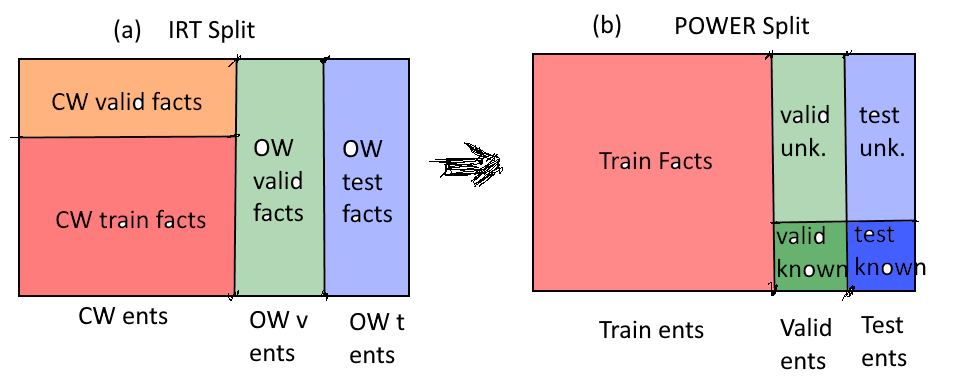
\includegraphics[width=\textwidth]{5_experiments/2_power_datasets/splits}
    \caption{Repartitioning an IRT fact split into a Power split by merging the train subsets and splitting validation and test subsets into facts are known and unknown during inference, respectively}
    \label{fig:5_experiments/2_power_datasets/splits}
\end{figure}

The percentage of known and unknown facts can be varied when creating the Power split to study the Ruler's effectiveness on entities with more or less given knowledge. Table~\ref{tab:5_experiments/2_power_datasets/power_splits} lists the splits used for the evaluation. In practice, few-shot splits are particularly interesting. Since there are only about 20 facts per entity on average, the fact splits with 5\% and 15\% known facts can be considered few-shot scenarios. The splits with 0\% known facts correspond to an zero-shot open-world scenario. For readability, the Power splits based on the CoDEx-M and FB15k-237 splits are abbreviate to "CDE" and "FB".

\begin{table}[h]
    \centering
    \begin{tabular}{| l | r | r | r | r | r |}
    \hline
    
    \multicolumn{1}{|c|}{\textbf{Power Split}} &
    \multicolumn{1}{|c|}{\textbf{\thead{Train Facts}}} &
    \multicolumn{1}{|c|}{\textbf{\thead{Known \\ Valid Facts}}} &
    \multicolumn{1}{|c|}{\textbf{\thead{Known \\ Valid Facts \\ per Entity}}} &
    \multicolumn{1}{|c|}{\textbf{\thead{Known \\ Test Facts}}} &
    \multicolumn{1}{|c|}{\textbf{\thead{Known \\ Test Facts \\ per Entity}}} \\

    \hline\hline

    CDE-0   & \multirow{6}{*}{\num{137738}} & \num{0}     & \num{0.00} & \num{0}     & \num{0.00} \\
    CDE-5   &                               & \num{2062}  & \num{0.71} & \num{1378}  & \num{0.73} \\
    CDE-15  &                               & \num{6186}  & \num{2.12} & \num{4136}  & \num{2.18} \\
    CDE-30  &                               & \num{12372} & \num{4.24} & \num{8273}  & \num{4.36} \\
    CDE-50  &                               & \num{20620} & \num{7.07} & \num{13788} & \num{7.27} \\
    CDE-100 &                               & \num{?}     & \num{7.07} & \num{13788} & \num{7.27} \\

    \hline

    FB-0   & \multirow{6}{*}{\num{238191}} & \num{0}     & \num{0.00}  & \num{0}     & \num{0.0} \\
    FB-5   &                               & \num{2325}  & \num{1.50}  & \num{1271}  & \num{1.56} \\
    FB-15  &                               & \num{6975}  & \num{4.51}  & \num{3813}  & \num{4.67} \\
    FB-30  &                               & \num{13950} & \num{9.03}  & \num{7626}  & \num{9.35} \\
    FB-50  &                               & \num{23251} & \num{15.05} & \num{12711} & \num{15.58} \\
    FB-100 &                               & \num{?}     & \num{15.05} & \num{12711} & \num{15.58} \\
    
    \hline
\end{tabular}

    \caption{Power splits with varying ratios of known test entities - for example, "CDE-50" denotes the CoDEx-M-based Power split with half of the test entities being known during inference while the FB-0 Power split does not reveal any of the FB15k-237 facts during inference}
    \label{tab:5_experiments/2_power_datasets/power_splits}
\end{table}



\section{Evaluation Metrics}
\label{sec:5_experiments/3_metrics}
When designing and implementing machine learning models, scientists act on experience when it comes to architectural decisions and hyperparameter choices. In the early stages of a model, a trained eye on processing examples and observing the loss curve enable rapid progress. However, as the model matures, it becomes essential to quantify its performance with respect to comprehensive validation and test sets. Besides the selection of appropriate validation and test data, it is important to choose a meaningful metric that fits the problem. For example, when all of a models predictions are equally relevant, one would aim for an overall high precision, whereas a use case that involves a human processing the results manually, such as a web search, for example, one would choose a ranking metric that rewards good results at the top of a list.

All considered metrics are defined by terms from the so-called confusion matrix shown in Figure~\ref{fig:2_basics/4_metrics/1_confusion_matrix}. The matrix applies to the general scenario in which predictions are made about a certain condition for a set of objects. Thereby, an object's actual condition can be positive or negative, also referred to as its \emph{ground truth}, as can be the object's predicted condition. A prediction is \emph{true}, or correct, if its predicted condition is consistent with the object's actual condition and \emph{false} otherwise. Furthermore, objects whose prediction is positive are called \emph{positives}, while objects whose predictions are negative are called \emph{negatives}. Depending on their actual and their predicted condition, each object falls into one of four distinct categories:

\begin{figure}[t]
    \centering
    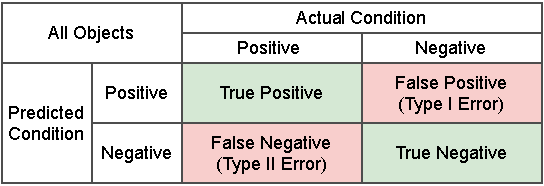
\includegraphics[width=\textwidth]{2_basics/4_metrics/confusion_matrix}
    \caption{Confusion Matrix dividing objects into four distinctive groups depending on their actual and predicted condition}
    \label{fig:2_basics/4_metrics/1_confusion_matrix}
\end{figure}

\begin{itemize}
    \item \textbf{\emph{True positives}} (TP) are objects for which the regarded condition is positive and whose predicted conditions is also positive.

    \item \textbf{\emph{False positives}} (FP) are objects for which the regarded condition is positive but whose predicted condition is negative. This type of error is referred to as a \emph{Type I error}.

    \item \textbf{\emph{False negatives}} (FN) are objects for which the condition is actually negative but whose predicted condition is positive. This second kind of errornous prediction is also referred to as \emph{Type II error}.

    \item \textbf{\emph{True negatives}} (TN) are objects for which the condition is actually negative and whose predicted condition is also negative.
\end{itemize}

Although it is generally desirable to obtain as many correct predictions as possible, true positives and true negatives are often differently important and errors of type one and two differently severe. In medicine, for example, not recognizing a disease could be much worse than accidentally diagnosing a healthy person as ill. Conversely, not recognizing guilt in a lawsuit might be less serious than convicting someone who is innocent. In the context of knowledge graph completion under the open-world assumption, the focus lies on true positives since the KGC model cannot make any qualified statements about false facts without negative samples in the graph. Omitting a fact from the prediction only means that the model has too little evidence for that fact, not that it can falsify it.

%The purpose of this section is to explain those metrics relevant for this work. Section~\ref{fig:2_basics/4_metrics/1_confusion_matrix} defines basic terms used by the following sections. Sections~\ref{subsec:2_basics/4_metrics/2_accuracy} and~\ref{subsec:2_basics/4_metrics/3_prf} then present the general purpose metrics accuracy, precision, recall and F1 score while Sections~\ref{subsec:2_basics/4_metrics/4_mrr} and~\ref{subsec:2_basics/4_metrics/5_map} discuss the ranking metrics MRR and mAP\@.

%\subsection{Confusion Matrix}
%\label{subsec:2_basics/4_metrics/1_confusion_matrix}
%All considered metrics are defined with the help of terms from a so-called confusion matrix as shown in Figure~\ref{fig:3_basics/4_metrics/1_confusion_matrix}. The matrix emerges from the general scenario in which predictions are made for a set of objects that can be either true or false. A prediction is true if its statement is consistent with reality about the object, also called ground truth, and false if the prediction contradicts reality. An example scenario would be an image recognition that has to determine whether a photo shows a cat or not. Then, four mutually exclusive types of predictions can be distinguished:

\begin{itemize}
    \item \textbf{\emph{True positives}} (TP) are predictions stating that a condition holds true when this is indeed the case. In the image recognition example, this would correspond to the case where the model correctly classifies a cat image as a cat.

    \item \textbf{\emph{False positives}} (FP) are negative predictions about objects where the condition is actually true, e.g. declaring an animal as cat although it is not. This type of error is also referred to as a \emph{Type 1 error}.

    \item \textbf{\emph{False negatives}} (FN) are another kind of erroneous predictions, also referred to as \emph{Type 2 errors}. They represent the case that an element with a true condition was classified as false - was overlooked, so to speak. An example would be a cat image not recognized as a cat.

    \item \textbf{\emph{True negatives}} (TN) are similar to true positives in that they are correct predictions, as well. They consist of rejective predictions about objects where the condition does indeed not apply, for example by recognizing that there is no cat in a cat-less photo.
\end{itemize}

Although it is generally desirable to obtain as many correct predictions as possible, true positives and negates are often differently important and errors of type one and two differently severe. In medicine, for example, not recognizing a disease could be much worse than accidentally diagnosing a healthy person as ill. Conversely, not recognizing guilt in a lawsuit might be less serious than convicting someone who is innocent. In the context of knowledge graph completion under the open-world assumption, the focus lies on true positives since the KGC model cannot make any qualified statements about non-applying facts without negative samples in the graph. Omitting a fact from the prediction only means that the model has too little evidence for that fact, not that it can falsify it.

\begin{figure}[t]
    \centering
    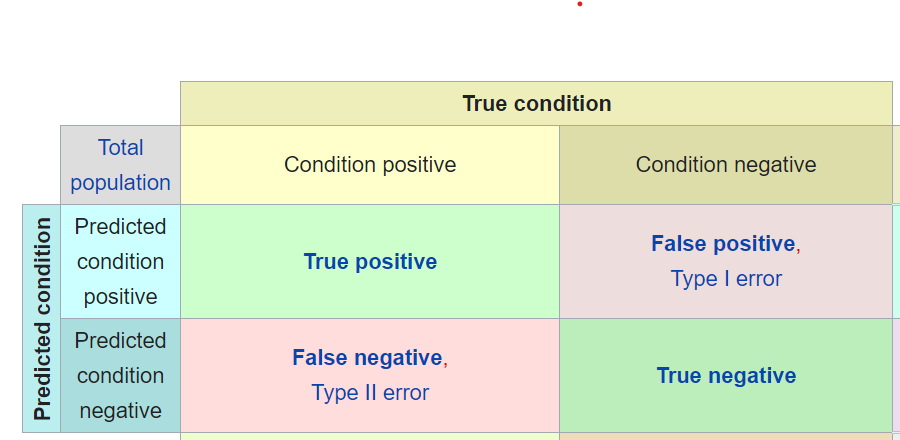
\includegraphics[width=\textwidth]{3_basics/4_metrics/1_confusion_matrix/matrix}
    \caption{Confusion Matrix}
    \label{fig:3_basics/4_metrics/1_confusion_matrix}
\end{figure}

"positive", "negative", "true", "false" predictions, "positive", "negative" elements

cat example
ir scenario


\subsection{Accuracy}
\label{subsec:2_basics/4_metrics/2_accuracy}
One of the most common general-purpose metrics is \emph{accuracy}, which measures a model's overall capability to make correct positive and negative predictions. In the case of binary classification, accuracy is the rate of correct predictions over all predictions:

\begin{align}
    Accuracy = \frac{TP + TN}{TP + TN + FP + FN}
    \label{eq:2_basics/2_metrics/1_accuracy/accuracy}
\end{align}

Colloquially speaking, accuracy answers the question of how good predictions are in general. It takes values in $[0, 1]$, whereby higher is better. However, although accuracy is a useful and intuitive metric in general, it can be misleading when it comes to unbalanced classes because a model can simply reach high accuracy by always predicting the predominant class. For example, if nine out of ten ground truth values are false, a model could reach 90\% accuracy by always predicting false. To counteract this, balanced accuracy~\cite{Mower2005PREPMtPR} can be used instead. However, as mention earlier, as negative predictions do not play a big role for KGC models in an open-world scenario, accuracy will only play a minor role in this work.


\subsection{Precision, Recall and F1}
\label{subsec:2_basics/4_metrics/3_prf}
\emph{Precision}, \emph{recall} and \emph{F1} focus on positive predictions. Precision gives an impression of how reliable positive predictions are, recall tells how many of the actual positive elements are declared as such, and F1 is a measure that combines both precision and recall in one value. All three metrics take values from $[0, 1]$ whereby higher is better.

Precision, also known as \emph{positive predictive value (PPV)}, is the ratio of true positive predictions to all positive predictions as noted in \autoref{eq:2_basics/2_metrics/2_prf/precision}. False negatives are not considered. If a model does not produce any predictions, precision is undefined and has to be defined in accordance with the evaluation scenario. One possibility is to define as 1 if the dataset does not contain any ground truth positives and 0 otherwise, because the model should not produce any predictions if, and only if, there are no ground truth positives.

\begin{align}
    Precision = \frac{TP}{TP + FP}
    \label{eq:2_basics/2_metrics/2_prf/precision}
\end{align}

Recall, on the other hand, also known as \emph{true positive rate (TPR)}, compares the number of true positives to the number of all ground truth positives as shown in \autoref{eq:2_basics/2_metrics/2_prf/recall}. False positives do not count in. If the evaluated dataset does not contain any ground truth positives, recall is undefined and might be specified as 1, because the model did not miss out on any ground truth positives.

\begin{align}
    Recall = \frac{TP}{TP + FN}
    \label{eq:2_basics/2_metrics/2_prf/recall}
\end{align}

Precision and recall are directly dependent on each other. A cautious model that only predicts positives when it is sure achieves high precision but low recall. Conversely, it is easy to achieve optimal recall by making positive predictions for all elements, though precision will suffer in that case. The \emph{F score} serves as a measure that considers both goals and reaches a high value when a reasonable balance between precision and recall is found. \autoref{eq:2_basics/2_metrics/2_prf/f_beta} shows the formula for the general $F_\beta$ score whose parameter $\beta$ determines whether the focus should rather be shifted towards precision or recall. Setting $\beta = 1$ yields the $F_1$ score in \autoref{eq:2_basics/2_metrics/2_prf/f_1} as the harmonic mean in which precision and recall are weighted equally.

\begin{align}
    F_\beta &= (1 + \beta^2) \cdot \frac{Precision \cdot Recall}{\beta^2 \cdot Precision + Recall}
    \label{eq:2_basics/2_metrics/2_prf/f_beta} \\
    F_1 &= 2 \cdot \frac{Precision \cdot Recall}{Precision + Recall}
    \label{eq:2_basics/2_metrics/2_prf/f_1}
\end{align}

Oftentimes, the predictions that should be made for a set of objects can be divided into subsets. For example, in a multi-label classification scenario, metrics can be calculated class-wise and when predicting facts for a set of entities, metrics can be calculated for each entity. In these cases there are multiple ways to calculate the metrics for the overall dataset:

\begin{itemize}
    \item Throw all predictions together and calculate the metrics over all predictions. This approach yields so-called \emph{micro} metrics, for example, micro precision.

    \item Calculate the metrics per subset, for example, class-wise, and specify the resulting values as such. This approach can yield detailed insights but potentially leads to many key figures.

    \item Calculate the metrics per subset and average the results, yielding \emph{macro} metrics.
\end{itemize}


\subsection{Mean Reciprocal Rank}
\label{subsec:2_basics/4_metrics/4_mrr}
The above presented accuracy, precision, recall and F1 metrics are useful in a classification task where no prioritization among the predictions is required. However, in an \emph{information retrieval (IR)} scenario, such as a web search, for example, a model might yield a sorted list of predictions where the ranking actually plays a major role. Usually, IR scenarios do not differentiate between positive and negative predictions, but rather between more or less relevant predictions that are returned by decreasing relevance.

In those cases it is more important to rank relevant items as high as possible among the overall results than it is assign the correct probability, or class if there is probability threshold, to each item. When it is most important to receive a correct top-most prediction for each query, the \emph{mean reciprocal rank (MRR)} is the metric of choice. Given the results of $n$ queries it is calculated as per \autoref{subsec:2_basics/2_metrics/3_mrr}, where $rank_i$ is the rank of the top-most relevant item among the predictions of the $i$th query results. Each reciprocal rank, and thus the mean over all reciprocal ranks, lies in $(0, 1]$, with higher being better. If a query result does not contain any relevant item, the reciprocal rank is undefined. Depending on the use case, the object might be skipped or assigned a specific value. A typical application scenario for MRR would be the evaluation of a voice assistant that has to respond with the single most relevant answer it gets from a model.

\begin{align}
    MRR = \frac{1}{n} \sum_{i=1}^{n} \frac{1}{rank_i}
    \label{eq:2_basics/2_metrics/3_mrr/mrr}
\end{align}


\subsection{Mean Average Precision}
\label{subsec:2_basics/4_metrics/5_map}
Another metrics that considers ranking is \emph{average precision (AP)}. In contrast to MRR it considers not only the top-most relevant result, but all of relevant results, including those not retrieved if the results are limited to a certain number. Given an object for which there are a set of relevant items $R$ and a model that predicts a set of items $P$, average precision is calculated as per Equation~\ref{eq:2_basics/4_metrics/5_map/ap}, in which $Prec@k$ is the precision among the first $k$ retrieved items and $rel@k$ is 1 if the $k$th item is relevant and 0 otherwise.

\begin{align}
    AP = \frac{1}{|R|} \sum_{k=1}^{|P|} Precision@k \cdot rel@k
    \label{eq:2_basics/4_metrics/5_map/ap}
\end{align}

Figure~\ref{fig:2_basics/4_metrics/4_mrr/mrr_map} illustrates the calculation of average precision by an example modeled after a possible list of facts predicted by the Power model when applied to the example entity Lisa from the graph in Chapter~\ref{ch:1_introduction}. Given the list of four predicted facts, sorted by confidence and covering two relevant facts, average precision for Lisa is calculated by adding up the $Precision@k$ values of the relevant facts and dividing the sum by the total number of relevant facts, including the one missing from the predictions.

\begin{figure}[t]
    \centering
    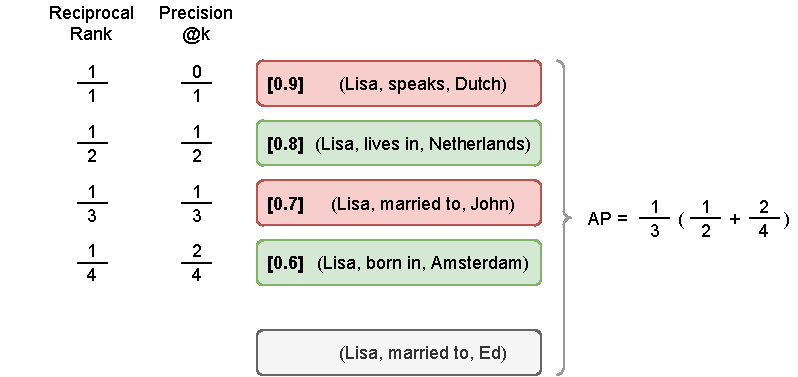
\includegraphics{2_basics/4_metrics/5_map/mrr_map}
    \caption{Calculation of average precision by example of a list of fact predictions, ranked by confidence and containing two of the totally three relevant facts - relevant facts are in green, irrelevant ones in red and the missed out relevant one in grey}
    \label{fig:2_basics/4_metrics/5_map/mrr_map}
\end{figure}

As for the MRR, mAP takes values in $(0, 1]$ and is not defined if there are no relevant items for an object. Again, the latter case might be handled by ignoring such objects. When evaluating $n$ objects, each with $AP_i$ with $1 <= i <= n$, \emph{mean average precision (mAP)} is calculated as the overall average value:

\begin{align}
    mAP = \frac{1}{n} \sum_{i=1}^{n} AP_i
    \label{eq:2_basics/4_metrics/5_map/map}
\end{align}






\section{Texter}
\label{sec:5_experiments/4_texter}
While the Ruler processes the query entity's known facts, the Texter takes the entity's sentences to predict facts. Although it can only predict the most common facts from the training set, its main advantage is its applicability to open-world entities that come without any known facts about them.

\subsection{Simple Model}
\label{subsec:4_approach/1_texter/1_simple_model}
During inference, the first step of processing a query entity, which is the same for both the simple and the attentive Texter, is embedding the entity's sentences in the embedding block. Thereby, each sentence is processed individually as illustrated in Figure~\ref{fig:4_approach/1_texter/1_simple_model/simple_architecture}: First, the sentence is split into words by the tokenizer, which are handled as integer IDs in further processing. Next, the words are embedded using some NLP approach, which could be a simple lookup table in the simplest case. As the last step in the embedding block, the word embeddings are combined to sentence embeddings in the pooling layer. The resulting sentence embeddings, that capture the sentences' overall meanings, are then passed on to the classification block where each of them is pushed through the neural multi-label classifier which consists of a single linear layer. Another pooling layer then combines the sentence-wise classification logits to the entity's logits. Finally, applying the sigmoid function to the entity's logits yields the class probabilites that state the probabilities of the associated facts about the query entity.

\begin{figure}[t]
    \centering
    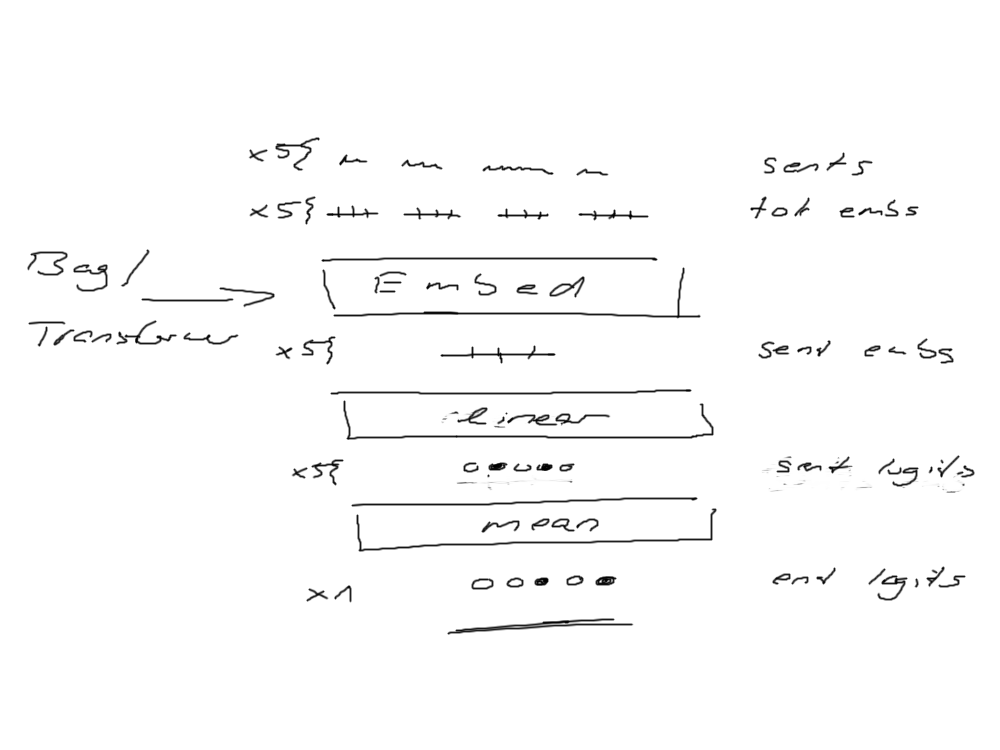
\includegraphics{4_approach/1_texter/1_simple_model/simple_architecture}
    \caption{Simple Texter Architecture; Each sentence is embedded and classified individually before the final pooling layer combines the results; "++++----" represents an embedding with positive and negative elements}
    \label{fig:4_approach/1_texter/1_simple_model/simple_architecture}
\end{figure}

Especially in the embedding block there are different possibilities for the concrete implementation of the individual parts to choose from, some of which will be examined in Chapter~\ref{ch:5_experiments}. In the final version of the power model, a transformer model is used for embedding the sentences' words, more precisely DistilBERT, a "distilled" variant of the transformer encoder BERT reduced to the essentials~\cite{Sanh2019DistilBERTAD}. In contrast to a simple lookup table, DistilBERT is able to incorporate the context of a word into its embedding, which leads to more meaningful sentence embeddings. This choice of embedding approach also affects the tokenizer, the pooling layer, and even the input sentences: Thanks to context embedding, transformers can use special tokens that add additional information to the text. While a classical model cannot decide on the basis of the sentence "Lisa likes John." whether this sentence speaks for the class $(x, has~gender, male)$, a transformer is able to do so given the appropriately marked sentence "Lisa likes [START]John[END].". Especially for long, ambigious sentences performance can be increased significantly.

Beyond the input data, the use of a transformer also affects the tokenizer and the pooling layer. The tokenizer has to apply byte pair encoding (BPE) that is commonly used by pre-trained transformers, where sentences are not only divided into words, but words are further divided into subwords, thus keeping the vocabulary of the tokenizer small and allowing to exploit homorphisms between similar words. In addition, the tokenizer inserts the [CLS] and [SEP] introduced by BERT at the beginning and end of the sentence. That way, "Lisa likes [START]John[END]." becomes "[CLS]Lisa likes [START]John[END].[SEP]". While the [SEP] token is used to separate sentences and has no further meaning here, the embedding of the [CLS] token captures the meaning of the whole sentence and is therefore  used as a sentence representation in the BERT paper~\cite{Devlin2019BERTPO}. However, the power experiments showed that performance can be increased if the word embeddings are also included, which is why the pooling layer of the embedding block averages all of a sentence's token embeddings, including the [CLS] embedding.

Less comprehensive processing steps happen in the classification block of the simple Texter: The sentence embeddings produced by the embedding block are pushed through the single linear classification layer whose multi-label output logits are averaged in the final pooling layer. The class probabilities calculated by applying the sigmoid function to the resulting entity logits are then used to sort the facts that have a probability greater than 50\%. Thus, the user of the model first receives the facts that are most likely to apply.


\subsection{Attention Model}
\label{subsec:4_approach/1_texter/2_attention_model}
While the simple Texter produces good evaluation results and does return a prioritized list of predicted facts, its prediction miss the desired explanation of why a fact is suggested. At this point, the attentive Texter extends the simple model by an attention mechanism that compares an entitiy's sentences to each other, forcing the model to favor sentences that are most relevant to the prediction of a certain fact. Besides the ability to provide an explanations for its predictions, the added attention mechanism should also increase the Texter's performance on datasets with multiple sentences per entity.

Technically, the attention mechanism is implemented as an attention block between the embedding and the classification blocks as shown in Figure~\ref{fig:4_approach/1_texter/2_attention_model/attention_architecture}. The embedding block is the same one used in the simple model, leveraging the DistilBERT encoder's contextual word embeddings to support marked input sentences and produce meaningful sentence embeddings. The classification block still produces the entity's multi-label output logits, but now uses multiple smaller linear layers to do so, due to the different outputs passed in from the attention block.

\begin{figure}[t]
    \centering
    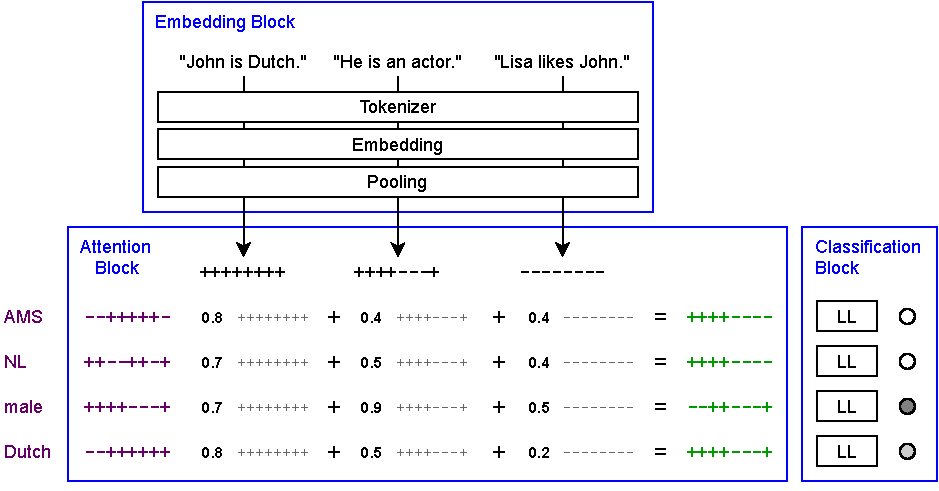
\includegraphics{4_approach/1_texter/2_attention_model/attention_architecture}
    \caption{Texter Architecture}
    \label{fig:4_approach/1_texter/2_attention_model/attention_architecture}
\end{figure}

The attention block now takes the sentence embeddings from the embedding block and compares them to so-called \emph{class embeddings} that represent each of the models output classes as a vector of the same dimension as the sentence embeddings. Given the set of input sentences $S$ and the set of classes $C$, the similarity between a class embedding $class_c$ and a sentence embedding $sent_s$ with $1 <= c <= |C|$ and $1 <= s <= |S|$ is calculated as the scalar product $\langle class_c, sent_s \rangle$ between the class and the sentece embedding. Given all class-sentence similarities for a certain class, the model can decide which sentence is matches the best for that class and deserves most attention when it comes to the decision whether the class holds true. Therefore, those similarity values are also referred to as attention values. To minimize the effect of sentences whose embeddings are very similar to a class embedding by pure chance, the attention values are furthermore normalized using the sigmoid function. Thus, the total attention matrix containing the attention values for all combinations of classes from $C$ and sentences from $S$ is calculated as shown in Equation~\ref{eq:4_approach/1_texter/2_attention_model/attention_matrix}.

\begin{align}
    A_{cs} = \sigma(\langle class_c , sent_s \rangle) && 1 <= c <= |C|, 1 <= s <= |S|
    \label{eq:4_approach/1_texter/2_attention_model/attention_matrix}
\end{align}

In the next step, the calculated attention values are used to combine the sentence embeddings to class-wise entity embeddings $ent_c$. As illstrated in Figure~\ref{fig:4_approach/1_texter/2_attention_model/attention_architecture} and formalized in Equation~\ref{eq:4_approach/1_texter/2_attention_model/ent_emb}, each sentence is thereby weighted by its class-wise attention value. The weighted sentences are then summed up to form class-wise entity embeddings whose purpose is to capture primarily those texts most relevant to the prediction of the respective class. Different from the simple Texter, the entity embeddings are then passed to the subsequent classification block instead of the original sentence embeddings.

\begin{align}
    ent_c = \sum_{s = 1}^{|S|} A_{cs} \cdot sent_s && 1 <= c <= |C|, 1 <= s <= |S|
    \label{eq:4_approach/1_texter/2_attention_model/ent_emb}
\end{align}

Similar to the simple Texter, the attentive Texter's classification consists of a $|C| \times d$ weight matrix and a bias vector of length $d$ where $d$ is the chosen embedding dimensionality for word, sentence, class and entity embeddings. In contrast to the simple model, however, given an entity embedding for a certain class, the weight matrix is not trained with respect to all output classes at once, but only with respect to the regarded class' ground truth output as illustrated in Figure~\ref{fig:4_approach/1_texter/2_attention_model/multi_linear}, which conceptually can be seen as training a separate single-output linear layer for each class and combining the outputs to the multi-label output thereafter. Formally, the models output classification outputs can be calculated as $out_c = \langle ent_c, W_c \rangle + b_c$ where $W_c$ and $b_c$ are the class' row in the weight matrix and its bias, respectively. The described approach to training the weight matrix was chosen, because a certain class' entity embedding focuses on the prediction of a single output class and would only hinder the learning process for other output classes it cannot make a qualified statement about.

\begin{figure}[t]
    \centering
    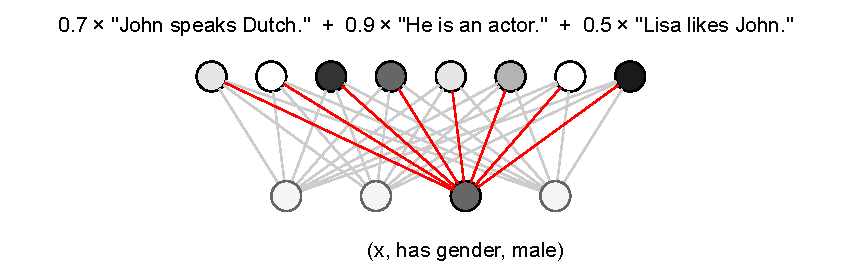
\includegraphics{4_approach/1_texter/2_attention_model/multi_linear}
    \caption{Multi-linear}
    \label{fig:4_approach/1_texter/2_attention_model/multi_linear}
\end{figure}

Similar to the simple Texter, following the core steps, the attentive Texter takes all classes whose confidences, that result from applying the sigmoid function to the output logits, is greater than 50\% to form their corresponding facts and sort them by confidence. In addition to the simple Texter, however, the attentive model provides the facts with the sentence weights as they result from the attention matrix in order to provide the user with an explanation for each fact's prediction. So, in the example, the fact $(John, has~gender, male)$, with a probability around 70\%, would be accompanied by the information that it was primarily suggested due to the sentence "He is an actor.", followed by "John speaks Dutch." and lastly "Lisa likes John.".

learnable class embs
sigmoid maps to (0, 1)
attention matrix A
total number of learnable params
in experiments: applied by an AdamW optimizer, a variant of the Adam optimizer that overcomes Adam's that keeps the training speed of Adam while keeping SGD's superior ability to generalize~, \cite{Loshchilov2019DecoupledWD}




\section{Ruler}
\label{sec:5_experiments/5_ruler}
While the Texter processes the text information attached to the knowledge graph's entities, the Ruler exploits patterns in the graph structure to predict missing facts. Given an entity $x$ with a set of known facts $K$ containing facts of the form $(x, rel_k, tail_k)$ with $1 <= k <= |K|$ and $rel_k \in R$ and $tail_k \in E$ being any relation or entity, respectively, the Ruler leverages entity-related rules of the form $(x, rel_m, tail_m) <= (x, rel_k, tail_k)$ with $1 <= m <= |M|$ to predict a set of missing facts $M$. Therefore, the rules required for the inference process have to be mined from the knowledge graph, beforehand. That rule mining process can be viewed as the equivalent to the Texter's training process and some paragraphs in this thesis will refer to combined rule mining and creation of a Ruler as "training" a Ruler. Compatibel to the Texter, the Ruler is limited to the prediction of facts $(x, rel, tail)$ that contain the query entity as their head, as well. However, when the Ruler is applied to all entities $e \in E$, all facts of the form $(e, rel, x)$ are predicted at some point as far as the mined rules support it.

For rule mining, AnyBURL, the bottom-up rule mining algorithm, by Christian Meilicke et al.~\cite{Meilicke2019AnytimeBR} is used. It is an anytime algorithm, meaning that it can be interrupted anytime and still yield valid results. Bottom-up rule mining refers to the fact that the algorithm starts with concrete paths in the graph and tries to generalize those paths to rules instead of coming up with rules initially and searching for evidence later, which would be a top-down approach. Out of all possible Horn rules that might describe patterns in the graph, AnyBURL is restricted to rules that can be generalized from so-called \emph{ground path rules}. A ground path rule does not contain variables, but only constants, and must not contain any cycles in its body. Equation~\ref{eq:4_approach/2_ruler/ground_path_rule} describes the general form of a ground path rule of length $n$, meaning that it consists out of the head fact and $n$ body facts.

\begin{align}
(c_0, h, c_1)
    \Leftarrow (c_1, b_1, c_2), \dots, (c_n, b_n, c_{n+1}) &&
    c_k \neq c_l \forall k, l \in \{1, \dots, n+1\}, k \ne l
    \label{eq:4_approach/2_ruler/ground_path_rule}
\end{align}

Notably, despite the rule body being free of cycles, the ground path rule as a whole can still be cyclic if $c_0 = c_{n+1}$. Ground path rules are derived directly from randomly sampled paths in the graph and are subsequently generalized to rules that replace some of the constants with variables. If further supporting paths can be found for a general rule, it is kept. In their paper on AnyBURL, Meilicke et al. show that any rule that can be generalized from a ground path rules can be generalized to one of the three rule types formulated in Equations~\ref{eq:4_approach/2_ruler/c}~--~\ref{eq:4_approach/2_ruler/ac2}. Thereby, $C$-type rules can only be generalized from cyclic ground path rules, $AC2$ rules can only be generalized from acyclic ground path rules and $AC1$ can be generalized from both, cyclic and acyclic ground path rules. The following paragraphs outline the core algorihm used to mine such rules and derive some example rules from the small graph introduced in Chapter~\ref{ch:1_introduction}. Figure~\ref{fig:4_approach/2_ruler/rule_graph} shows an annotated subset of the graph that illustrates the rules. "Amsterdam" and "Netherlands" have been abbreviated to "AMS" and "NL" to keep the examples short.

\begin{align}
    C   && (Y, h, X)   &\Leftarrow (X, b_1, A_2), \dots, (A_n, b_n, Y)
    \label{eq:4_approach/2_ruler/c} \\
    AC1 && (c_0, h, X) &\Leftarrow (X, b_1, A_2), \dots, (A_n, b_n, c_{n+1})
    \label{eq:4_approach/2_ruler/ac1} \\
    AC2 && (c_0, h, X) &\Leftarrow (X, b_1, A_2), \dots, (A_n, b_n, A_{n+1})
    \label{eq:4_approach/2_ruler/ac2}
\end{align}

\begin{figure}[t]
    \centering
    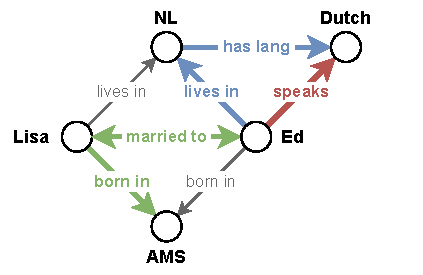
\includegraphics{4_approach/2_ruler/rule_graph}
    \caption{Subset of the previously introduced example graph with highlighted facts that form an acyclic (red + green) and a cyclic (red + blue) path.}
    \label{fig:4_approach/2_ruler/rule_graph}
\end{figure}

Essentially, AnyBURL repeatedly samples random paths from the graphs, generalizes them to all possible rule types, looks for further paths that match the gained rules, and keeps those rules it finds further evidence for. For example, in search of rules of length 2, i.e. rules that have a body consisting of 2 facts, AnyBURL might randomly sample the two paths in~\ref{eq:4_approach/2_ruler/path_1} and~\ref{eq:4_approach/2_ruler/path_2} from the graph. Note, that parentheses denote entities, brackets denote relations and that the path does not need to follow directed edges in the graph. Furthermore, a close look at the paths reveals that the second path is cyclic as it starts and ends at the entity "Dutch".

\begin{align}
(Dutch)
    \leftarrow [speaks] - (Ed) - [married~to] \rightarrow (Lisa) - [born~in] \rightarrow (AMS)
    \label{eq:4_approach/2_ruler/path_1} \\
    (Dutch) \leftarrow [speaks] - (Ed) - [lives~in] \rightarrow (NL) - [has~lang] \rightarrow (Dutch)
    \label{eq:4_approach/2_ruler/path_2}
\end{align}

From those paths, AnyBURL would then derive the constant-only
ground path rules~\ref{eq:4_approach/2_ruler/acyclic_ground_path} and~\ref{eq:4_approach/2_ruler/cyclic_ground_path} by taking the path's first part as the rule's head and the remaining parts to form the rule's body.

\begin{align}
(Ed, speaks, Dutch)
    &\Leftarrow (Ed, married~to, Lisa), (Lisa, born~in, AMS)
    \label{eq:4_approach/2_ruler/acyclic_ground_path} \\
    (Ed, speaks, Dutch) &\Leftarrow (Ed, lives~in, NL), (NL, has~lang, Dutch)
    \label{eq:4_approach/2_ruler/cyclic_ground_path}
\end{align}

The acyclic ground path rule in~\ref{eq:4_approach/2_ruler/acyclic_ground_path} can be generalized to the $AC1$ rule~\ref{eq:4_approach/2_ruler/acyclic_ac1} and the $AC2$ rule~\ref{eq:4_approach/2_ruler/acyclic_ac2} while the cyclic ground path rule~\ref{eq:4_approach/2_ruler/cyclic_ground_path} can be generalized to the $C$ rule~\ref{eq:4_approach/2_ruler/cyclic_c} and the $AC1$ rule~\ref{eq:4_approach/2_ruler/cyclic_ac1}.

\begin{align}
    AC1 && (X, speaks, Dutch) &\Leftarrow (X, married~to, A_2), (A_2, born~in, AMS)
    \label{eq:4_approach/2_ruler/acyclic_ac1} \\
    AC2 && (X, speaks, Dutch) &\Leftarrow (X, married~to, A_2), (A_2, born~in, A_3)
    \label{eq:4_approach/2_ruler/acyclic_ac2} \\
        C   && (X, speaks, Y) &\Leftarrow (X, lives~in, A_2), (A_2, has~lang, Y)
    \label{eq:4_approach/2_ruler/cyclic_c} \\
    AC1 && (X, speaks, Dutch) &\Leftarrow (X, lives~in, A_2), (A_2, has~lang, Dutch)
    \label{eq:4_approach/2_ruler/cyclic_ac1}
\end{align}

Next, every rule candidate is scored by looking for further paths that match the rule's body and checking whether the graph also contains the fact predicted by the rule, i.e. whether the rule is correct in that case. Thereby, the number of paths that match the rule body is called the rule's \emph{support} while the ratio of times the rule is correct over its total support is called \emph{confidence}. Taking the cyclic rule~\ref{eq:4_approach/2_ruler/cyclic_c} as an example, AnyBURL would search for further evidence and find the path $(Lisa) - [lives~in] -> (NL) - [has~lang] -> (Dutch)$ that matches the rule body, increasing the rule's support to two, so far. However, the example graph does not contain the rule's predicted fact $(Lisa, speaks, Dutch)$, so the rule's support drops from 1 to $\frac{1}{2}$. Since rules that only apply to a single case or only once in every thousands case are not very useful, AnyBURL drops rules with a support of 1 or confidence below 0.0001 by default~\cite{AnyBURL}. It is noteworthy that, although some rules are more general than others, such as~\ref{eq:4_approach/2_ruler/acyclic_ac2} compared to~\ref{eq:4_approach/2_ruler/acyclic_ac1}, the more specific ones are still kept as they might end up with higher confidence for their special case during the ongoing mining process.

The process described by the above example is repeated until only few new rules of the same length $n$ can be found. AnyBURL then continues its search for rules of length $n + 1$ until it terminates after a fixed number of time steps. Listing~\ref{code:anyburl} shows the slightly adjusted pseudocode from the AnyBURL paper. The sampling and scoring process discussed above is implemented as the body of the inner while loop. The outer for loop implements the repeated check for the saturation of rules of the current length and the eventual proceeding to rules of increased length.

% TODO param s

\begin{listing}[t]
    \begin{lstlisting}
        AnyBURL(G, sat, Q, i, ts):
            n = 2
            R = $\emptyset$
            for i times:
                $R_s = \emptyset$
                start = current_time()
                while current_time() < start + ts:
                    p = sample_path(G, n)
                    $R_p$ = generate_rules(p)
                    for $r$ in $R_p$:
                        score($r$)
                        if $Q$($r)$:
                            $R_s$ = $R_s \cup {r}$

                $R_s^{'}$ = $R_s \cap R$
                if $|R_s^{'}| / |R_s| > sat$:
                    n = n + 1
                $R$ = $R \cup R_s$

            return $R$
    \end{lstlisting}
    \caption{The AnyBURL rule mining algorithm takes a graph $G$, a saturation level $sat$, a quality criterion $Q$, and a number of iterations $i$, each of a timespan $ts$, as input and produces a ruleset $R$.}
    \label{code:anyburl}
\end{listing}

A walk through the pseudocode reads as follows: Given the Graph $G$, the saturation threshold $s$, the quality criterion $Q$, a number of iterations $i$ and the timespan $ts$ each iteration endures, AnyBURL starts with an empty ruleset $R$, that will be extended after each iteration and returned in the end. The initial length of the randomly sampled paths is $n=2$, allowing to find the shortest possible rules of length 1. During the first iteration of duration $ts$, AnyBURL fills the rule set $R_s$, that keeps the rules found in the current iteration, by repeatedly sampling paths, generating rules from the paths, scoring the resulting rules, and keeping those with sufficient support and confidence. At the end of the iteration, when the timespan $ts$ has passed, $R_s^{'}$ is calculated as the set of rules mined during the iteration that were already known. If the share of already known rules mined during the current iteration exceeds the saturation threshold, the algorithm starts searching for rules of increased length. Otherwise, it continues with the current length. In both cases, the iteration's rules are added to the overall ruleset $R$. If the specified number of total iterations is reached, AnyBURL terminates and returns the mined rules $R$. In practice, AnyBURL saves the mined rules in a text file at the end and at configurable points during mining.

With the stored rules from AnyBURL in place, the Ruler is prepared for inference. Conceptually, given an entity and its known facts, the Ruler loads the rules, filters out further rules that do not meet the Ruler's quality demands and applies the remaining, useful rules to all known facts. All rules that can be applied successfully are kept together with their confidence. From all the facts predicted by the applied rules, already known facts from the existing graph are filtered out. The remaining facts are sorted by confidence and returned to the user - together with the rules that predicted them as an explanation for the user. If multiple rules predict the same fact, the fact is assigned the highest confidence of those rules and is returned together with all of them. The Ruler's extra quality criterion mentioned above further restricts the considered rules to those with confidence greater 50\%, because AnyBURL's minimum confidence threshold of 0.01\% allows many rules that predict false positives. For open-world entities, this algorithm implies an empty result set as no rule can cover an entity that is not connected to any other entity and all the facts predicted for the train entities will be filtered out. In those cases, the Power model has to rely solely on the Texter.



\section{Aggregator}
\label{sec:5_experiments/6_aggregator}
The aggregator has the task of merging the predicted facts from Ruler and Texter. As envisioned in \autoref{sec:4_approach/3_aggregator} and illustrated in \autoref{fig:4_approach/3_aggregator/lucy}, it was hoped that merging the facts leads to higher average precision because facts predicted by both components are likely to be correct and should be ranked higher. In addition, the Aggregator should be able to estimate how reliable the predictions of Ruler and Texter are in relation to each other, which is implemented in the form of the weight parameter $\alpha$ as described in \autoref{eq:4_approach/3_aggregator/conf_aggregator}.

\autoref{tab:5_experiments/5_aggregator/results} shows the final evaluation results for the Aggregator, and thus the final evaluation results for the Power model, for a number of graph-text combinations. As fact splits, the splits with 50\% known test facts were chosen, as for the final Ruler evaluation in \autoref{sec:5_experiments/4_ruler}. The respective results for the CDE-50 and FB-50 splits from \autoref{tab:5_experiments/4_ruler/results} were taken over into \autoref{tab:5_experiments/5_aggregator/results} for easier comparability. Similarly, the chosen text sets are the ones from the final Texter evaluation in \autoref{subsec:5_experiments/3_texter/3_context}. Again, \autoref{tab:5_experiments/5_aggregator/results} duplicates the respective results from \autoref{tab:5_experiments/3_texter/3_context/results} for ease of comparison. The last two columns then contain the new Aggregator measurements for the combination of the corresponding Ruler and Texter.

\begin{table}[t]
    \makebox[\textwidth][c]{
        \begin{tabular}{ l l c r r r }
    \toprule

    \multicolumn{1}{l}{\textbf{Text Set}} &
    \multicolumn{1}{l}{\textbf{Texter}} & \phantom &
    \multicolumn{3}{c}{\textbf{Macro over Classes}} \\

    \cmidrule{4-6}

    & 
    &&
    \multicolumn{1}{c}{\textbf{Prec}} &
    \multicolumn{1}{c}{\textbf{Rec}} &
    \multicolumn{1}{c}{\textbf{F1}} \\
    
    \midrule

    \multirow{2}{*}{cde-cde-1-clean}
    & Simple    && \textbf{49.02} & 47.57 & 47.67 \\
    & Attentive && 46.86 & \textbf{51.09} & \textbf{47.98} \\

    \addlinespace

    \multirow{2}{*}{cde-irt-1-clean}
    & Simple    && 25.20 & \textbf{34.18} & \textbf{28.13} \\
    & Attentive && \textbf{26.70} & 31.41 & 27.43 \\

    \addlinespace

    \multirow{2}{*}{cde-irt-5-clean}
    & Simple    && 36.49 & \textbf{44.38} & \textbf{38.98} \\
    & Attentive && \textbf{39.20} & 37.11 & 36.98 \\

    \addlinespace

    \multirow{2}{*}{cde-irt-15-clean}
    & Simple    && 41.83 & \textbf{48.69} & \textbf{44.07} \\
    & Attentive && \textbf{44.63} & 37.39 & 39.78 \\

    \addlinespace

    \multirow{2}{*}{cde-irt-30-clean}
    & Simple    && 40.73 & \textbf{50.09} & \textbf{44.11} \\
    & Attentive && \textbf{43.60} & 36.10 & 38.78 \\
    
    \midrule

    \multirow{2}{*}{fb-owe-1-clean}
    & Simple    && 42.36 & \textbf{86.72} & 54.03 \\
    & Attentive && \textbf{45.21} & 84.03 & \textbf{56.16} \\

    \addlinespace

    \multirow{2}{*}{fb-irt-1-clean}
    & Simple    && 26.40 & 46.68 & 32.51 \\
    & Attentive && \textbf{27.01} & \textbf{49.90} & \textbf{34.26} \\

    \addlinespace

    \multirow{2}{*}{fb-irt-5-clean}
    & Simple    && 34.37 & \textbf{55.95} & 40.88 \\
    & Attentive && \textbf{39.21} & 50.63 & \textbf{43.50} \\

    \addlinespace

    \multirow{2}{*}{fb-irt-15-clean}
    & Simple    && \textbf{48.95} & \textbf{54.85} & \textbf{50.06} \\
    & Attentive && 48.89 & 52.75 & 49.92 \\

    \addlinespace

    \multirow{2}{*}{fb-irt-30-clean}
    & Simple    && 43.90 & \textbf{63.31} & \textbf{50.55} \\
    & Attentive && \textbf{50.57} & 48.47 & 48.79 \\
    
    \bottomrule
\end{tabular}

    }
    \caption{Final Aggregator results, i.e. final results for the Power model. The results of the Ruler and Texter, whose predictions the Aggregator combines, are also shown for comparison. Although the Aggregator does not outperform its respective Ruler and Texter in terms of F1 score, it does for mAP.}
    \label{tab:5_experiments/5_aggregator/results}
\end{table}

As the mAP values show, the Aggregator performs several percentage points better than the Ruler and Texter on their own, with the improvement on the CDE split being more obvious. However, the relatively small increase on the FB split suggests that the true positives of Ruler and Texter almost coincide there. For the CDE split, on the other hand, manually peeking into the predictions reveals that the improved mAP mainly results from complementary true positives -- and not so much from improved ranks of joint predictions. Looking at the values of simple and attentive Texter, it is also noticeable that the lead of the simple Texter over the attentive Texter shrinks when adding the Ruler. Likewise, the lead of the text sets with many sentences and with high-quality sentences shrinks. Finally, the different aptitudes for Ruler and Overall, the Aggregator results are even similar between the two splits, while previously, models performed significantly better on the FB split.

Two experiments that will be mentioned only briefly here, because of their unspectacular results, concerning the calculation of the Aggregator's confidence as per \autoref{eq:4_approach/3_aggregator/conf_aggregator}: First, in the beginning, experiments were conducted on the computation of the combined confidence $conf_{Aggregator}$ in cases where facts are predicted by Ruler and Texter. As combining methods, calculating the maximum and the mean of $conf_{Ruler}$ and $conf_{Texter}$ were evaluated, but it soon became apparent that summing them up much better accommodates the fact that a fact predicted by Ruler and Texter deserves very high confidence. Second, experiments showed that taking into account the weight parameter $\alpha$ between Ruler and Texter yields only marginal performance improvements in the tenths of a percent range because the confidence values of Ruler and Texter seem to be very comparable after all and thus always yield $\alpha$ values close to 0.5. In detail, Ruler and Texer were both a bit too optimistic about their predictions in the experiments -- but they were equally overconfident.

